\documentclass[11pt]{article}
\usepackage[margin=0.85in]{geometry}
\usepackage{amsmath,amssymb,graphicx,xurl,hyperref}
\setlength{\parindent}{0pt}\setlength{\parskip}{7pt}
\begin{document}
{\LARGE Integral modular Hermite accumulator}\par
November9,2026. Mathematical source \texttt{15ab03e54}. Unsigned producer
evidence throughout [pcc:unverified].

\textbf{Construction.} For the actual source grid and orders, put
\[
 K=8h2^a+8M(a+1),\qquad h=\lceil3M/u\rceil.
\]
Every actual node's child-precision overhead is at most $K$. Applying the
existing coefficient-error theorem at output precision zero, then multiplying
by the remaining nonnegative power of two, establishes
\[
 g_{t,j}=2^K E_t(0)(-t/\alpha)^j\in\mathcal O\quad(j<q_t).
\]
Here $\mathcal O$ is the concrete rational two-adic integral subring. Define
\[
 G(J)=\sum_t\sum_{j<q_t}g_{t,j}J_{t,j}\in\mathcal O.
\]
Lean identifies its rational value with $2^K$ times the actual Hermite
recovery functional for the prescribed quotient degrees.

\textbf{Cross-precision transition.} The actual residue kernel is $(2^p)$.
Divisibility cancellation in the integral domain therefore gives
\[
 [2^Kx]_{p+K}=[2^Ky]_{p+K}\iff[x]_p=[y]_p.
\]
No inverse of two in a fixed finite-characteristic ring is assumed.
For the actual computed finite quotient buffers, the scaled accumulator has
\[
 [G(J)]_{p+K}=\left[2^K\sum_xA_xB_x\right]_{p+K}.
\]
The target is not an input to the functional. Domain: integral rational weights,
$3\leq u\leq a$, $u\leq M$, injective supplied placement. $p$ is bit precision.

\textbf{Representation scope.} A finite sum admits fold evaluation, so its
algebra does not require retaining every node's quotient vector simultaneously.
Native low-bit extraction, efficient coefficient/input-jet construction, peak
retained state and recomputation costs remain unproved. This is an algebraic
streaming bridge, not measured memory savings or a recursive cost theorem.
\newpage
{\Large Dependencies and checks}\par
\begin{center}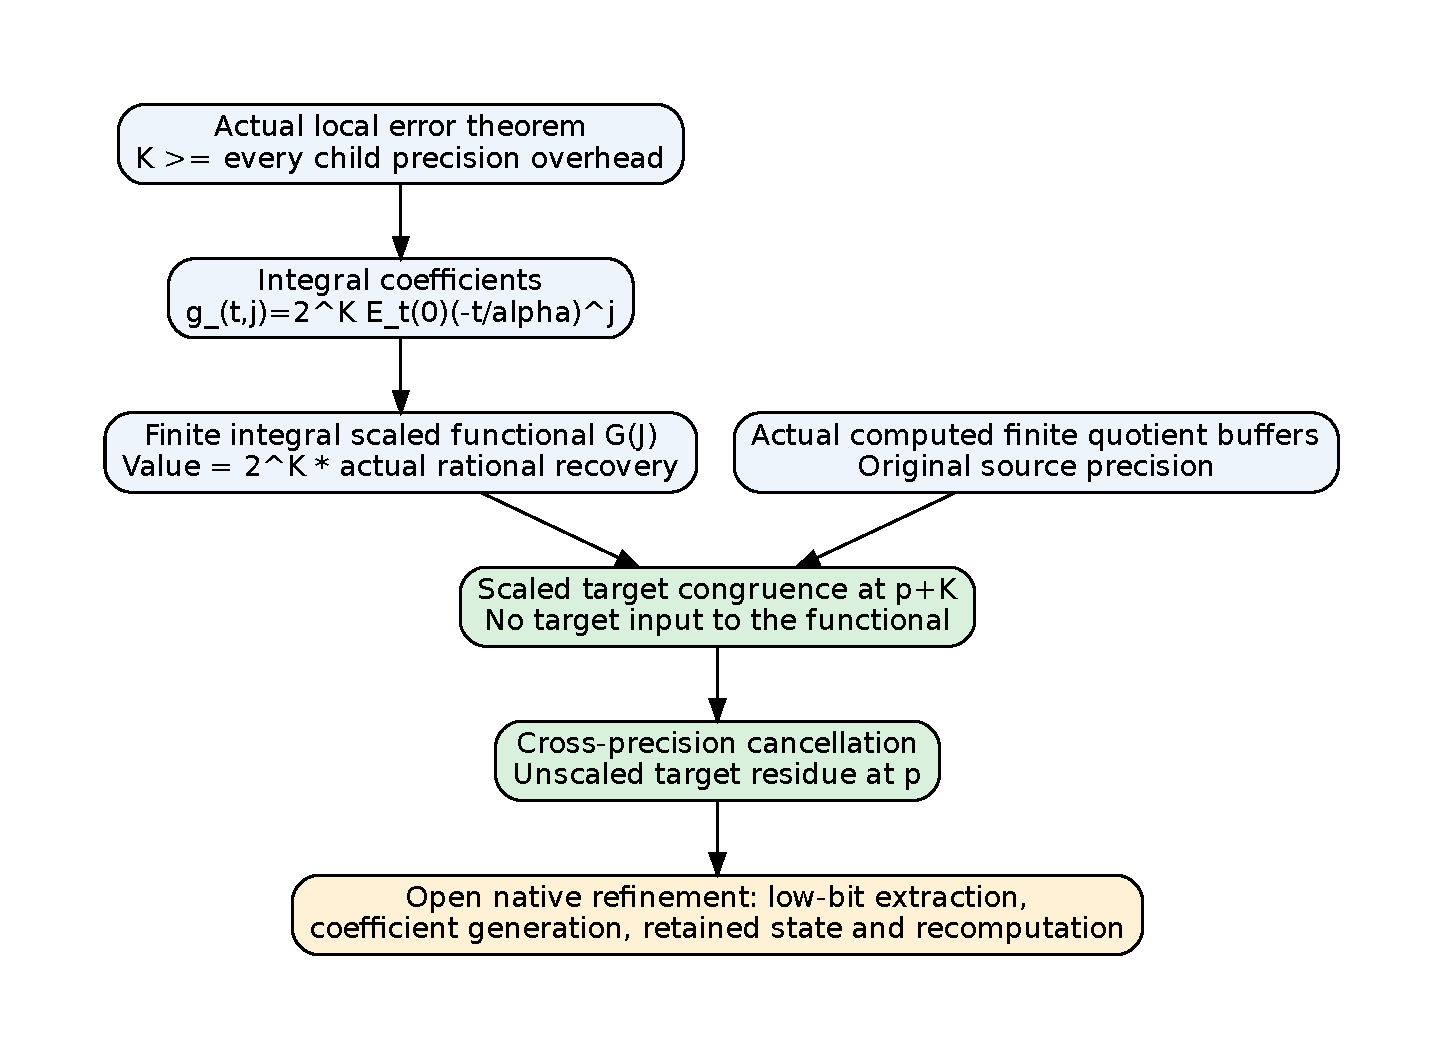
\includegraphics[width=0.95\linewidth,height=0.61\textheight,keepaspectratio]{stream.pdf}\end{center}

Five canonical unsigned PCC bindings (prefix \texttt{PCC-20261109-}):
residue equivalence9fdb17; cross-precision cancellation445413; actual scaled
coefficient integrality d2a76b; scaled-functional mapping f27d83; actual computed
scaled target residue eb2e7e. Canonical hashes, successful and failed build logs,
and final audit/replay receipts are retained beside the Lean sources and linked
in the companion Markdown report.

Sources: actual residue kernel, actual Hermite coefficient-error theorem,
constructed finite recovery and the pinned manuscript D.9/D.10 cited in the
preceding report. KB unavailable; no novelty assertion. A native accumulator
arm requires a prospective amendment to the currently frozen census. No census,
timing or memory measurement is reported in this phase.
\end{document}
